\subsection{Component Identification in Figure T-2}
\label{T6C07}

\begin{tcolorbox}[colback=gray!10!white,colframe=black!75!black,title=T6C07]
    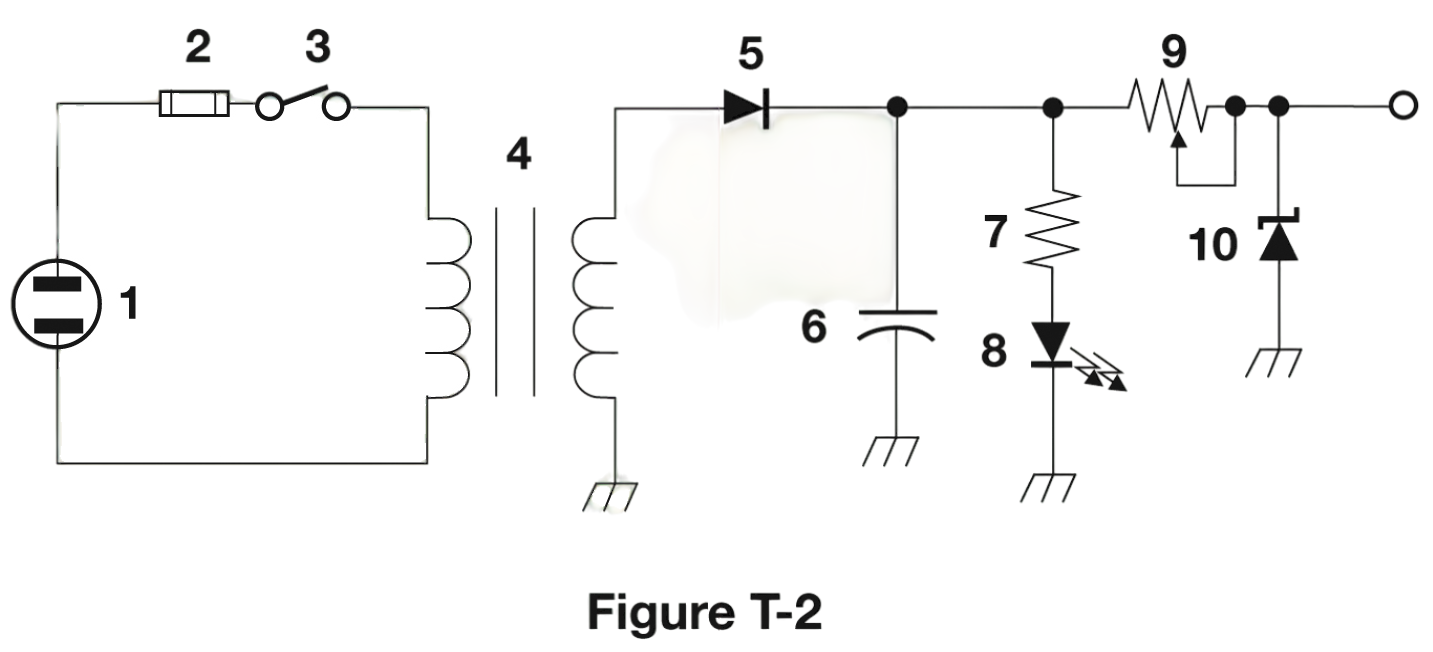
\includegraphics[width=0.5\textwidth]{tech/images/t2.png} 

    What is component 8 in figure T-2?


\begin{enumerate}[label=\Alph*)]
    \item Resistor
    \item Inductor
    \item Regulator IC
    \item \textbf{Light emitting diode}
\end{enumerate}
\end{tcolorbox}

\subsubsection{Intuitive Explanation}
Imagine you’re looking at a circuit board, and you see a tiny little light that blinks when the circuit is on. That’s component 8! It’s like the little flashlight of the circuit, telling you, “Hey, I’m working!” So, when you see that light, you know it’s a Light Emitting Diode, or LED for short. It’s not a resistor, inductor, or some fancy regulator chip—it’s just the circuit’s way of saying, “I’m alive!”

\subsubsection{Advanced Explanation}
In electronic circuits, a Light Emitting Diode (LED) is a semiconductor device that emits light when an electric current passes through it. The LED is characterized by its forward voltage drop, typically around 1.8V to 3.3V, depending on the material used. The current through the LED must be limited by a resistor to prevent damage. In the context of figure T-2, component 8 is identified as an LED based on its symbol and typical placement in circuits. The symbol for an LED is similar to a diode but includes arrows pointing away from the diode, indicating light emission.

% Prompt for generating the diagram:
% Include a diagram of figure T-2 with component 8 clearly labeled as an LED. The diagram should show the circuit layout and the symbol for the LED.